\section{Results and Discussion}
\label{sec:results}

\subsection{The period-\teff\ relations, revealed}
\label{sec:the_reveal}

To explore the relationship between rotation period, effective temperature
(\teff ) and velocity dispersion, we calculated \sigmavb \footnote{\sigmavb
was calculated as 1.5$\times$ the median absolute deviation, to mitigate
sensitivity to outliers.} for groups of stars with similar rotation periods
and temperatures, and presumed similar age.
The top panel of figure \ref{fig:vplot} shows rotation period versus effective
temperature for the \mct\ sample, coloured by \sigmavb, where \sigmavb\ was
calculated for groups of stars over a grid in $\log_{10}$(period) and
temperature.
If we assume that mass dependent heating does not strongly affect this sample
and \vb\ at low galactic latitudes is an unbiased tracer of \vz, then \vb\
velocity dispersion can be interpreted as an age proxy, and stars plotted in a
similar color in figure \ref{fig:vplot} are similar ages.
We discuss this assumption further in the appendix.
\begin{figure}
  \caption{
    Top: Rotation period vs effective temperature for stars in the \mct\
    sample, colored by the velocity dispersions of stars calculated over a
    grid in $\log_{10}$(period) and \teff.
    Black lines show gyrochrones from a gyrochronology model that projects the
    rotation-color relation of
    Praesepe to longer rotation periods over time \citep{angus2019}.
    These gyrochrones do not appear to reflect the evolution of field stars at
    long rotation periods/old ages because they do not trace lines of constant
    velocity dispersion.
    Gyrochrones are plotted at 0.5, 1, 1.5, 2, 2.5, 4 and 4.57 Gyr in both top
    and bottom panels.
    Bottom: Same as top panel with rotation period vs {\it mass}
    \citep[from][]{berger2020}.
    White lines show gyrochrones from a model that includes mass and
    age-dependent angular momentum transport between the core and envelope
    \citep{spada2019}.
    Qualitatively, these gyrochrones reflect the evolution of field
    stars at long rotation periods/old ages: they trace lines of constant
    velocity dispersion by reproducing periods of `stalled' rotational
    evolution for K-dwarfs.
}
  \centering
    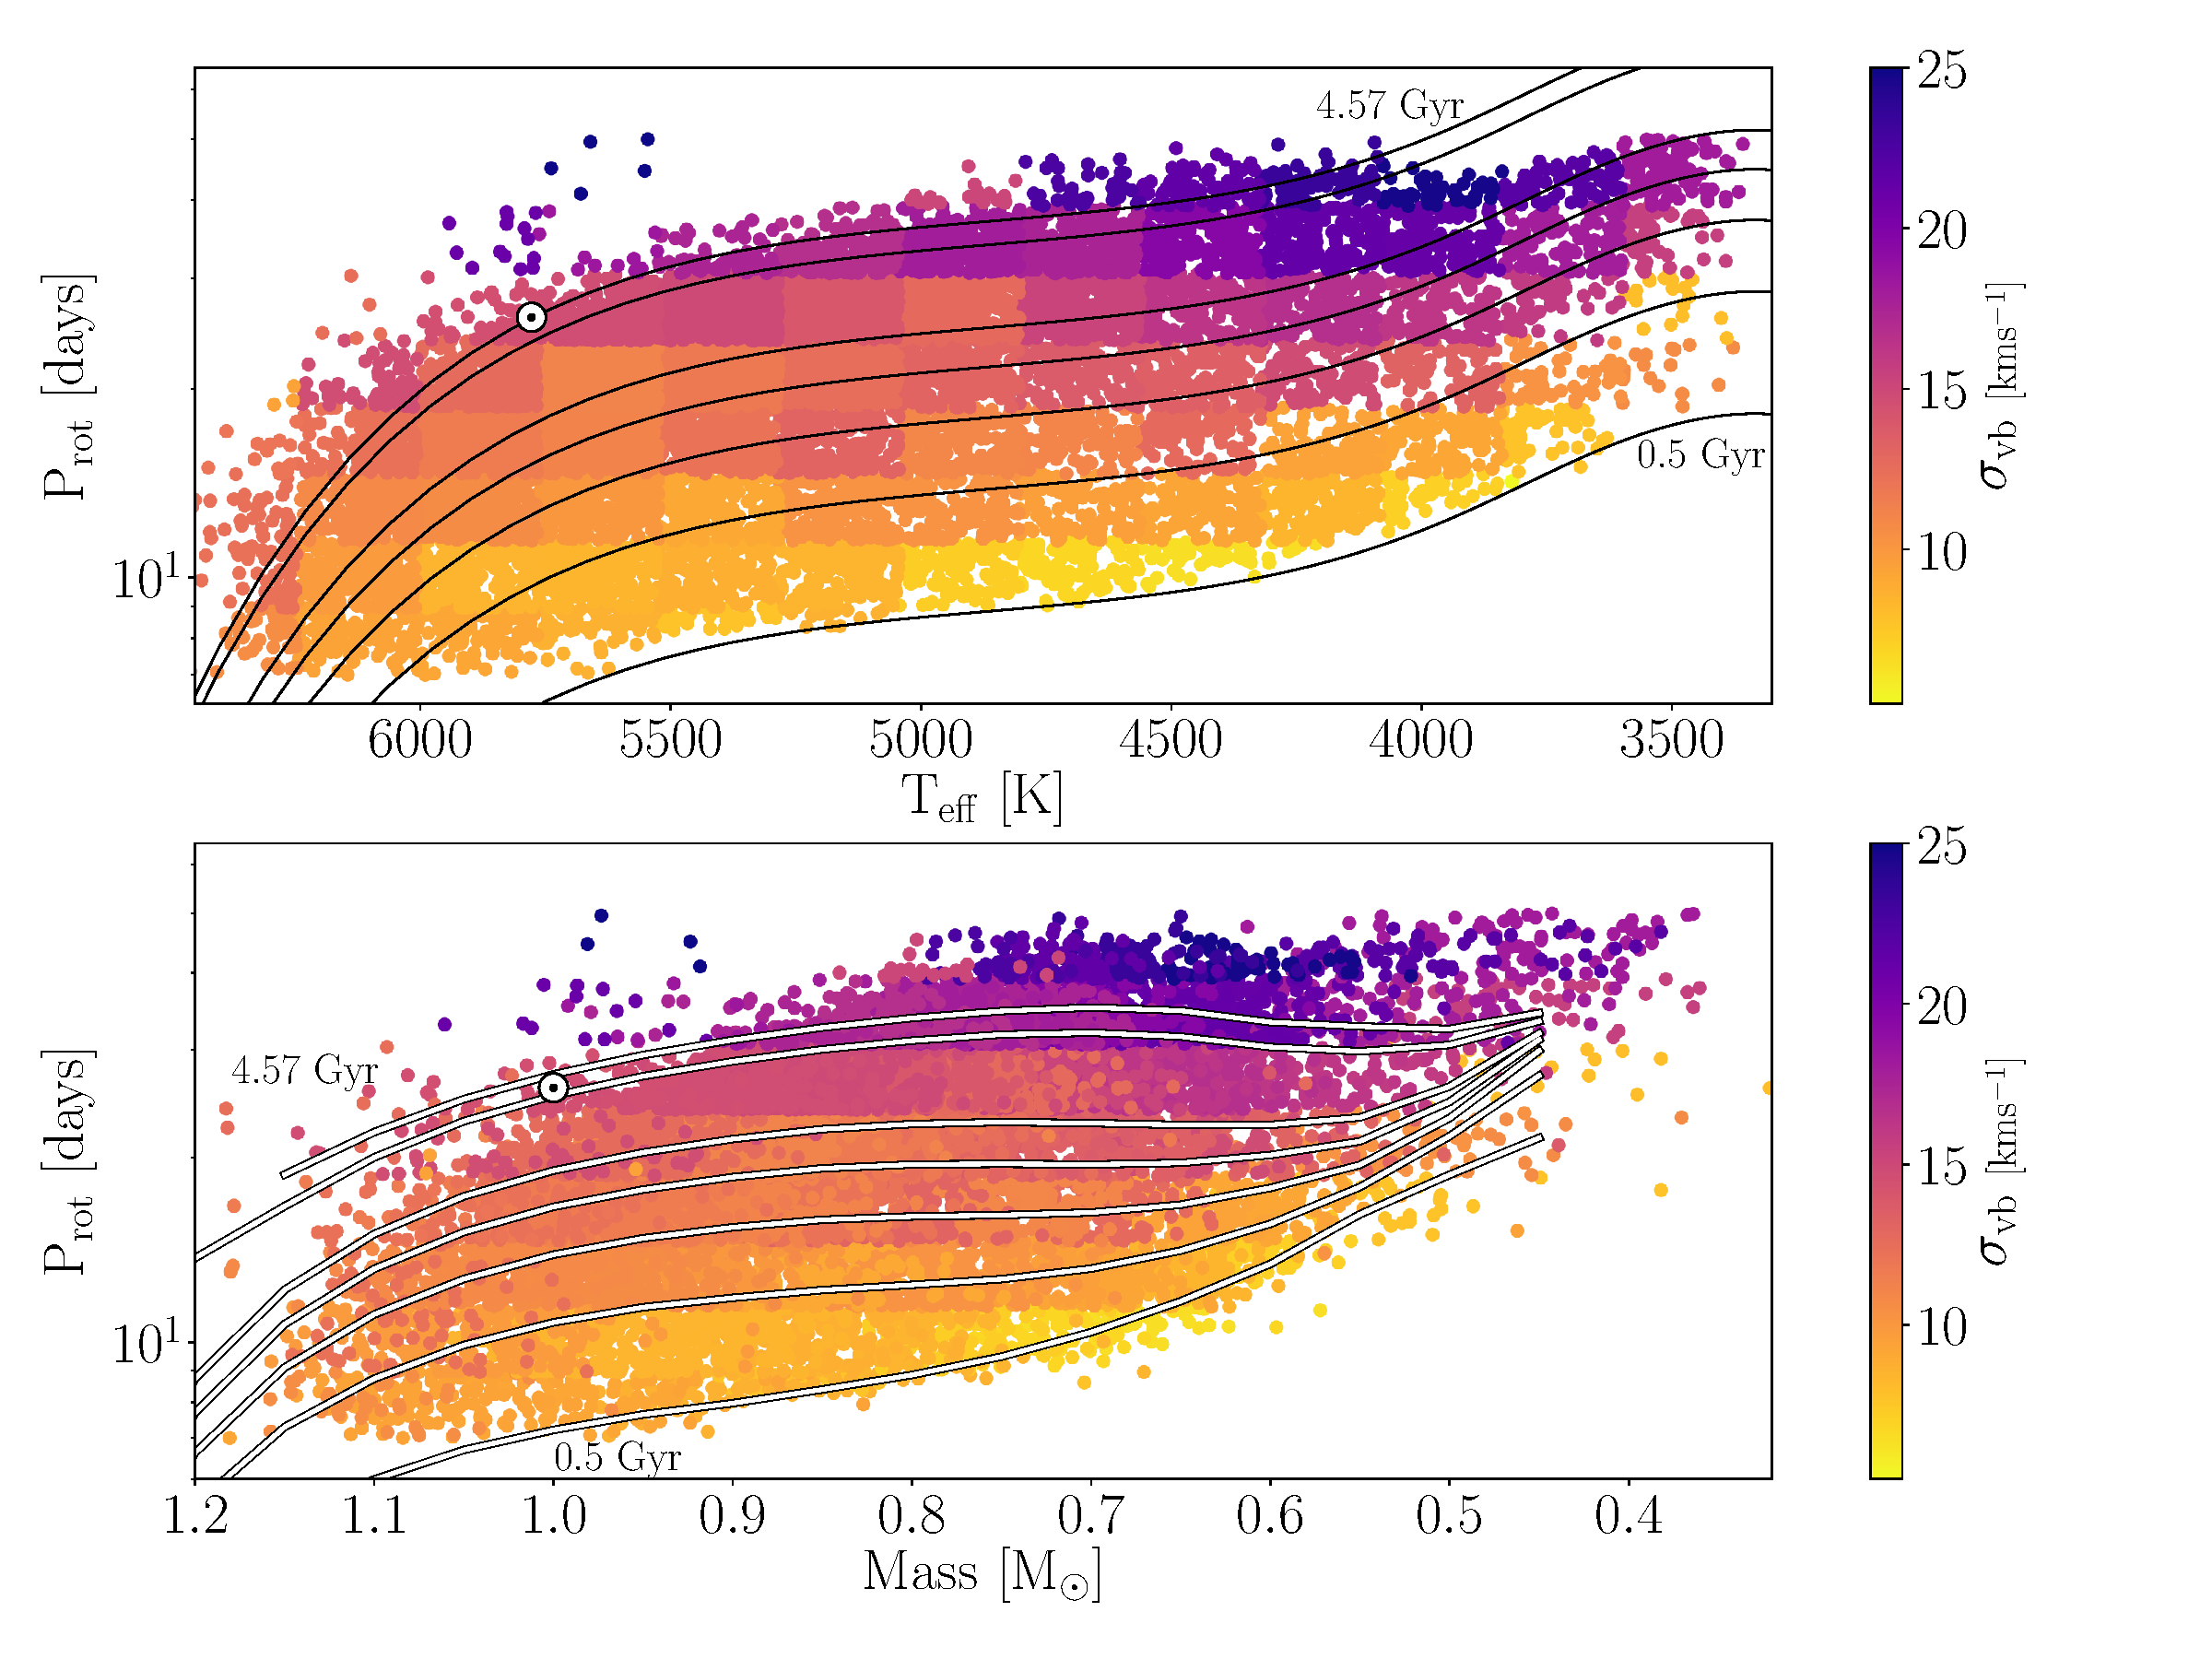
\includegraphics[width=1\textwidth]{main_figure}
\label{fig:vplot}
\end{figure}

Overall, figure \ref{fig:vplot} shows that velocity dispersion increases with
rotation period across all temperatures, implying that rotation period
increases with age, as expected.
This result is insensitive to the choice of bin position and size.
Black lines show gyrochrones from the \citet{angus2019} gyrochronology model,
which projects the rotation-color relation of Praesepe to longer rotation
periods over time.
These gyrochrones are plotted at 0.5, 1, 1.5, 2, 2.5, 4 and 4.57 Gyr.
At the youngest ages, these gyrochrones describe the data well: the palest
yellow (youngest) stars with the lowest velocity dispersions all fall close to
the 0.5 Gyr gyrochrone.
However, although the 0.5 Gyr and 1 Gyr gyrochrones also trace constant
velocity dispersion/age among the field stars, by 1.5 Gyr the gyrochrones
start to {\it cross} different velocity dispersion regimes.
For example, the 1.5 Gyr gyrochrone lies on top of stars with velocity
dispersions of around 10-11 kms$^{-1}$ at 5000-5500K and stars with $\sim$15
\kms\ velocity dispersions at 4000-4500K.
The gyrochrones older than 1.5 Gyr also cross a range of velocity dispersions.
If these were true isochrones they would follow lines of constant velocity
dispersion.
At ages older than around 1 Gyr, it appears that gyrochrones should have a
more flattened, or even inverted, shape in rotation period-\teff\ space than
these Praesepe-based models.

The bottom panel of figure \ref{fig:vplot} shows velocity dispersion as a
function of rotation period and {\it mass}, \citep[from][]{berger2020}, with
gyrochrones from the \citep{spada2019} model shown in white.
These gyrochrones are also plotted at 0.5, 1, 1.5, 2, 2.5, 4 and 4.57 Gyr.
Each point plotted in the top panel also appears in the bottom panel with the
same color.
Because velocity dispersion was calculated in bins of \teff, not mass, bin
outlines are clearly visible in the top panel but appear smeared-out in the
bottom panel.
In the bottom panel of figure \ref{fig:vplot}, the \citet{spada2019} models
{\it do} trace lines of constant velocity dispersion, and reproduce the trends
in the data at all ages.
These models qualitatively agree with the data and reproduce the apparent
flattening and inversion in the rotation period-\teff/mass relations.

The results shown in figure \ref{fig:vplot} indicate that stars of spectral
type ranging from late G to late K ($\sim$5500-3500 K) follow a braking law
that changes over time.
In particular, the relationship between rotation period and effective
temperature appears to flatten out and eventually invert.
These results provide further evidence for `stalled' rotational evolution of K
dwarfs, like that observed in open clusters \citep{curtis2019} and reproduced
by models that vary angular momentum transport between stellar core and
envelope with time and mass \citep{spada2019}.
The velocity dispersions of stars in the \mct\ sample provide the following
picture of rotational evolution.
At young ages \citep[younger than around 1 Gyr but still old enough to be on
the main sequence and have transitioned from the `I' sequence to the `C'
sequence ][]{barnes2003}, stellar rotation period {\it decreases} with {\it
increasing} mass.
This is likely because lower-mass stars with deeper convection zones have
stronger magnetic fields, larger Alfv\'en radii and therefore experience
greater angular momentum loss rate \citep[\eg][]{schatzman1962, parker1970,
kawaler1988, charbonneau2010}.
According to the \citet{spada2019} model, there is minimal transportation of
angular momentum from the surface to the core of the star at these young ages,
so the surface slows down but the core keeps spinning rapidly.
This aligns with the current assumptions about stellar spin-down, dynamo
theory, and the gyrochronology paradigm that has been in place for decades
\citep[\eg][]{skumanich1972, noyes1984, kawaler1988, barnes2003, angus2019}.
According to the data presented in figure \ref{fig:vplot} however, at
intermediate ages, the rotation periods of K dwarfs appear {\it constant} with
mass, and at late ages rotation period {\it increases} with {\it increaasing}
mass.
The interpretation of this, according to the \citet{spada2019} model, is that
lower-mass stars are still braking more efficiently at these intermediate and
old ages but their cores are more tightly coupled to their envelopes, allowing
angular momentum transport between the two layers.
Angular momentum resurfaces and prevents the stellar envelopes from
spinning-down rapidly, and this effect is strongest for late K-dwarfs with
effective temperatures of $\sim$4000-4500K and masses $\sim$0.5-0.7 M$_\odot$.

It has been demonstrated that lower-mass stars remain magnetically active
longer than more massive stars, \citep[\eg][]{west2008, kiman2019}.
If the detectability of a rotation period is considered to be a magnetic
activity proxy, then our results provide further evidence for a mass-dependent
activity lifetime.
Figure \ref{fig:vplot} shows that the groups of stars with the largest
velocity dispersions are cooler than 4500 K.
This implies that the oldest stars with detectable rotation periods, are
cooler than 4500 K, \ie\ these-low mass stars stay active longer than more
massive stars.

\subsection{Synchronized binaries and the \kepler\ period gap}
\label{sec:gap}

\begin{figure}
  \caption{
      Top: rotation period vs. effective temperature for stars in the \mct\
    sample, separated into three groups. Blue circles
      show stars with rotation periods longer than the
    period gap, orange squares show stars with rotation periods shorter than
    the gap, but longer than the lower edge of the main rotation period
    distribution, and green triangles show stars with rotation periods shorter
    than this lower edge.
    Stars were separated into these three groups using \citet{angus2019}
    gyrochronology models, with the scheme shown in the legend.
    Only stars cooler than 5000 K are plotted in
    the bottom panel in order to isolate populations above and below the
    period gap, which only extends up to temperatures of $\sim$4600 K.
    Bottom: the velocities of these groups of stars (in the direction of
    Galactic latitude, $b$) are shown as a function of rotation period.
    The black line indicates the velocity standard deviation as a function of
    period.
}
  \centering
    \includegraphics[width=1\textwidth]{gap}
\label{fig:gap}
\end{figure}

In this section, we explored the kinematic properties of the \mct\ sample in
more detail, investigating the velocity dispersions of stars either side of the
\kepler\ period gap, and identifying rapidly rotating stars that may be
synchronized binaries.

There is a sharp gap in the population of rotation periods (often called the
\kepler\ period gap), which lies just above the 1 Gyr gyrochrone in the upper
panel of figure \ref{fig:vplot}, whose origin is unknown and is the subject of
much speculation \citep{mcquillan2014, davenport2018, reinhold2019}.
This gap was first identified by \mct, and roughly follows a line of constant
gyrochronal age of around 1.1 Gyr \citep[according to the][gyrochronology
relation]{angus2019}.
Several explanations for the gap's origin have been proposed, including a
discontinuous star formation history \citep{mcquillan2013, davenport2017,
davenport2018} and a change in magnetic field structure causing a brief period
where rotational variability is reduced and rotation periods cannot be
measured \citep{reinhold2019}.

The top panel of figure \ref{fig:vplot} suggests that the \citet{angus2019},
Praesepe-based gyrochronology model is valid below the gap but not above.
Gyrochrones follow lines of constant velocity dispersion below the gap, but
{\it cross} lines of constant velocity dispersion above the gap.
Although we do not provide an in-depth analysis here (and more data may be
needed to confirm a connection) these data suggest that the gap may indeed
separate a young regime where stellar cores are decoupled from their envelopes
from an old regime where these layers are more tightly coupled.
If so, this could indicate that the phenomenon responsible for changing the
shape of gyrochrones in rotation-\teff\ space is related to the phenomenon that
produces the gap.

An alternate explanation for the gap is that the \mct\ sample contains two
distinct stellar populations: one young and one old.
If so, the kinematic properties of stars above and below the gap are likely to
be distinctly different.
The bottom panel of figure \ref{fig:gap} shows the velocity dispersions of
stars in the \mct\ sample, with stars subdivided into three groups: those that
rotate more quickly than the main rotation period population (green
triangles), those with rotation periods shorter than the gap (orange squares),
and those with rotation periods longer than the gap (blue circles).
Stars were separated into these three groups using \citet{angus2019}
gyrochronology model, according to the scheme shown in the legend.
Only stars cooler than 5000 K are included in the bottom panel in order to
isolate populations above and below the period gap, which only extends up to a
temperature of $\sim$4600 K in our sample \citep[Although][found that the gap
extends to temperatures as hot as 6000 K]{davenport2017}.
In general, velocity dispersion increases with rotation period because both
quantities increase with age.
There is a smooth transition in velocity dispersion between stars with
rotation periods below and above the gap (orange squares to blue circles),
suggesting that these groups are part of the same Galactic population.
Previously, only the overall velocity dispersions of all stars above and below
the gap have been compared, leading to the assumption that these groups belong
to two distinct populations \citep{mcquillan2014}.
The smooth increase in velocity dispersion across the gap shown here supports
the hypothesis that the gap is caused by a phenomenon of magnetic or
structural stellar evolution, not a discontinuity in the local star formation
history.

Synchronized binaries are pairs of stars whose rotation periods are equal to
their orbital period.
Since synchronization appears to happen at rotation periods of 7 days or
shorter \citep{simonian2019}, and most isolated stars have rotation periods
longer than 7 days, the rotation periods of synchronized binaries are likely
to be {\it shorter} than they would be if they were isolated stars.
For this reason, their rotation periods do not reflect their ages and the
gyrochronal age of a synchronized binary is likely to be much younger than the
true age of the system.
Synchronized binaries are therefore a source of contamination for
gyrochronology and should be removed from samples before performing a
gyrochronal age analysis.
Figure \ref{fig:gap} shows that some of the most rapidly rotating stars in the
\mct\ sample have relatively large absolute velocities, indicating that they
are likely synchronized binaries.
For this reason, the velocity dispersions of stars with rotation periods
shorter than the lower edge of the rotation period distribution (green
triangles in figure \ref{fig:gap}) are not significantly smaller than the,
presumed older, orange-colored stars.
In general, stars with rotation periods less than $\sim$10 days have an
increased chance of being synchronized binaries.
This result is in agreement with a recent study which found that a large
fraction of photometric binaries were rapid rotators, and the probability of a
star being a synchronized binary system substantially increased below rotation
periods of around 7 days \citep{simonian2019}.
We caution users of rotation period catalogs that rapid rotators with large
absolute velocities should be flagged as potential synchronized binaries
before applying any gyrochronal analysis.
